\documentclass[tikz]{standalone}

% \usepackage{newtxtext,newtxmath}
%!TEX root = main.tex

% mytikzset
\usepackage{tikz}
\usetikzlibrary{positioning,arrows,shapes,patterns}
\usetikzlibrary{decorations.pathmorphing}
\usetikzlibrary{decorations.markings}
\usetikzlibrary{decorations.pathreplacing}
\usetikzlibrary{calc}
\usetikzlibrary{patterns}
\usetikzlibrary{decorations.markings}
\usetikzlibrary{petri}

\tikzset{
  vector/.style={thick,double,draw=black, postaction={decorate},
    decoration={markings,mark=at position .6 with {\arrow[black,scale=0.4]{triangle 45}}}},
  axial/.style={thick,double,densely dashed,draw=black, postaction={decorate},
    decoration={markings,mark=at position .6 with {\arrow[black,scale=0.4]{triangle 45}}}},
  gluon/.style={decorate, draw=black,
    decoration={coil,aspect=0.3,segment length=5pt,amplitude=3pt}},
  pseudo/.style={thick, dashed, draw=black, postaction={decorate},
    decoration={markings,mark=at position .6 with {\arrow[red,scale=0.5]{triangle 45}}}},
  scalar/.style={thick,draw=black, postaction={decorate},
    decoration={markings,mark=at position .6 with {\arrow[black,scale=0.5]{triangle 45}}}},
  cut/.style={draw=black, decorate, decoration={snake, segment length=1mm, amplitude=0.2mm}}
}


\definecolor{cola}{rgb}{0.9,0.62,0.0}
\definecolor{colb}{rgb}{0.337, 0.706, 0.914 }
\definecolor{colc}{rgb}{0.0, 0.62, 0.451}

\begin{document}
\nopagecolor
  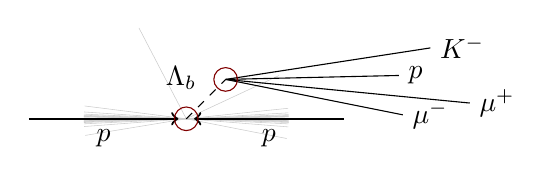
\begin{tikzpicture}[node distance=0.9cm and 1.3cm, baseline=1cm]
%
    \foreach \a in {-10,-8.7,...,10} :
      \draw[very thin, black!20!white] (0, 0) -- ({10/\a}:1.3)  ;
    \foreach \a in {-10,-8.77,...,10} :
      \draw[very thin, black!20!white] (0, 0) -- ({180+10/\a}:1.3);
%
    \draw[->,thick] (-2, 0) -- node[below] {$p$} (-0.1, 0);
    \draw[->,thick] ( 2, 0) -- node[below] {$p$} (0.1 ,0);
%
    \node[coordinate] (vLb) at (0.5 ,0.5) {};
    \draw[dashed]   ( 0, 0) -- node[above left] {$\Lambda_b$} (vLb);
    \draw[] (vLb) -- (2.7, 0.55) node[right] {$p$};
    \draw[] (vLb) -- (3.1, 0.9) node[right] {$K^-$};
    \draw[] (vLb) -- (3.6, 0.2) node[right] {$\mu^+$};
    \draw[] (vLb) -- (2.75, 0.05) node[right] {$\mu^-$};
    % \draw[] (vLb)--(0.5,0.5) -- ++(0.5,0.5) rectantular;
%
    % \draw[] (vLb) -- (3.75, 0.1) node[right] {$\gamma$};
    % \draw[] (0,0) -- (2.7, -0.3) node[right] {$\pi^+$};
    % \draw[] (0,0) -- (2.9, -0.5) node[right] {$\pi^-$};
%
    \draw[red!50!black] (vLb) circle (1.5mm);
    \draw[red!50!black] (0,0) circle (1.5mm);
  \end{tikzpicture}
\end{document}
